\chapter{Hypothesis Testing and Model Selection}
Hypothesis testing (also known as model selection, particularly when it is
done using the method in Section~\ref{sec:marginal_likelihood})
is a very important topic that is traditionally considered
a different topic from parameter estimation. However, in Bayesian statistics
we will see that hypothesis testing is basically the same thing as parameter
estimation! The one difference, for us, will be that we will sometimes change
the prior distribution a little bit.

One big advantage of Bayesian statistics is that it {\it unifies}
parameter estimation and hypothesis
testing\footnote{``Unifies'' is a popular word for physicists. It means that
two seemingly different topics are fundamentally the same, or at least closely
related.}. That's good news, because instead of having to
understand two different topics, we only have to understand one!

To see why hypothesis testing is fundamentally the same as parameter estimation,
you only need to
understand how parameter estimation works from a Bayesian point of view, which
we have already studied.
Parameter estimation is nothing more than testing a bunch of hypotheses about
the value of the parameter. For example, $\theta=1$ vs. $\theta=2$ vs. $\theta=3$ and
so on. If we have their posterior probabilities, then we've tested them.

\section{An Example Hypothesis Test}
Suppose we were performing a Bayesian parameter estimation analysis using a
Bayes' Box. Here is an example Bayes' Box with made up numbers:

\begin{table}[!ht]
\begin{center}
\begin{tabular}{|c|c|c|c|c|}
\hline
\tt{possible values} & \tt{prior} & \tt{likelihood} & \tt{prior} $\times$ \tt{likelihood} & \tt{posterior}\\
$\theta$ & $p(\theta)$ & $p(x|\theta)$ & $p(\theta)p(x|\theta)$ & $p(\theta|x)$\\
\hline
1.5 & 0.25 & 0.2 & 0.05 & 0.1\\
2.0 & 0.25 & 0.4 & 0.1 & 0.2\\
2.5 & 0.25 & 0.6 & 0.15 & 0.3\\
3.0 & 0.25 & 0.8 & 0.2 & 0.4\\
\hline
Totals & 1 & & 0.5 & 1\\
\hline
\end{tabular}
\end{center}
\end{table}
Suppose we wanted to test the following two hypotheses about the parameter $\theta$.
The first hypothesis $H_0$ is a ``null hypothesis'', and the second hypothesis,
$H_1$, is an ``alternative hypothesis''.
\begin{eqnarray}
H_0: && \theta = 2\\
H_1: && \theta \neq 2
\end{eqnarray}
In classical statistics, if you saw a question phrased in this way, you would
need to come up with a {\it test statistic}
and then calculate a {\it p-value}, which tries to say something about whether
the value of the test statistic would be considered extreme, under the
assumption that $H_0$ is true.
In Bayesian statistics, the only thing we need to do is calculate
the posterior probability of $H_0$ and the posterior probability of $H_1$.
The posterior probability of $H_0$ is given by:
\begin{eqnarray}
P(H_0|x) &=& P(\theta = 2|x)\\
&=& 0.2
\end{eqnarray}
All we did here was look up the appropriate number in the Bayes' Box! The
posterior probability of $H_1$ is only slightly harder (but still easy)
to calculate: $H_1$ will
be true if $\theta$ takes any value other than 2. Therefore, the posterior
probability of $H_1$ is
\begin{eqnarray}
P(H_1|x) &=& P(\theta = 1.5 \textbf{ or } \theta = 2.5 \textbf{ or } \theta = 3|x)\\
&=& P(\theta = 1.5|x) + P(\theta = 2.5|x) + P(\theta = 3|x)\\
&=& 0.1 + 0.3 + 0.4\\
&=& 0.8.
\end{eqnarray}
Here we used the fact that everything in a Bayes' Box is mutually exclusive
(only one of the hypotheses is true) so we could add the probabilities.
Alternatively, you could have just noticed that $H_1$ is true if $H_0$ is false.
So $P(H_0|x) + P(H_1|x) = 1$, which implies $P(H_1|x) = 1 - P(H_0|x)$.

\section{The ``Testing'' Prior}
Here we will study a hypothesis testing example that involves a null and an
alternative hypothesis. Since the bus example has been used a lot, we will now
switch over to a different example.

Suppose it is known that the mean systolic blood pressure
in the general population is 120 mm Hg, with a standard deviation of
15 mm Hg (millimetres of mercury is an
old fashioned unit for pressure, even though it sounds like a unit of length).
A new drug is developed that may
be helpful in reducing blood pressure. A sample of $N=100$ people
(who can be considered representative of the general population)
are given the drug, and their systolic blood pressure is measured. This results
in 100 blood pressure measurements $\{x_1, x_2, ..., x_N\}$, which will be
our data. As a shorthand, I'll sometimes write $\boldsymbol{x}$
(a bold vector) to denote the data collectively,
instead of $\{x_1, x_2, ..., x_N\}$.

We are interested in whether the drug works. Let $\mu$ be the mean systolic
blood pressure
that would apply in the general population if everyone was taking the
drug. Our goal is to infer the value of $\mu$ from the data. In classical
statistics, this is sometimes phrased as a hypothesis test between the two
competing hypotheses. We will not be concerned with the possibility that the
drug has the opposite effect to what is intended.
\begin{equation}
\begin{array}{ll}
H_0: & \mu = 120 \textnormal{ (the drug does nothing)}\\
H_1: & \mu < 120 \textnormal{ (the drug reduces blood pressure)}
\end{array}
\end{equation}
Suppose the mean of all the data values was
\begin{eqnarray}
\bar{x} &=& \frac{1}{N} \sum_{i=1}^{100} x_i\\
&=& 115.9.
\end{eqnarray} % and (x squared)bar = 13654.82
Does this data provide evidence against $H_0$ and in favour of $H_1$? In
classical statistics this question would be addressed using a {\it p-value}.
The p-value would be the probability of getting a result this extreme or
a result more extreme than what is observed, assuming that the ``null hypothesis''
is true. That is,
\begin{eqnarray}
\textnormal{p-value} = P(\bar{x} \leq 115.9 | H_0).
\end{eqnarray}
In case you're curious, the p-value in this case is 0.0031, which is usually
taken to mean that there is fairly strong evidence against $H_0$ and in favour
of $H_1$. To calculate the p-value I had to assume that the probability distribution
for the data values $\{x_1, x_2, ..., x_{100}\}$ was a normal distribution
with a known standard deviation of $\sigma=15$, and
that they were independent:
\begin{eqnarray}
x_i \sim \mathcal{N}(\mu, \sigma^2). \label{eq:normal}
\end{eqnarray}

In Bayesian statistics, p-values are not used. Instead, we should think of this
as a parameter estimation problem. We can state a set of hypotheses about the
value of $\mu$, and then choose a prior distribution, update to a posterior
distribution, etc. Then our result will be the posterior probability of the
null hypothesis, $P(H_0 | \boldsymbol{x}) = P(\mu = 120 | \boldsymbol{x})$.
This is helpful because the posterior probability of the null hypothesis is
exactly what we want. It is a description of how plausible the null hypothesis
is given the data. It is not some other probability that isn't really relevant.
We can also get the posterior probability of $H_1$ by summing the posterior
probabilities for all other values of $\mu$ apart from 120, or by using
$P(H_1 | \boldsymbol{x}) = 1 - P(H_0 | \boldsymbol{x})$.

There is only one minor tweak we need to make to make Bayesian inference an
appropriate framework for solving this problem. When the null and alternative
hypotheses are written like we wrote them above, it implies that the value of $\mu$
that we are calling the ``null hypothesis'' is a {\it special value that is
especially plausible}. To take this into account in our Bayesian analysis we
need to make sure the prior distribution recognises there is a special
value of the parameter that we think is extra plausible. When we do this, we
will call it a {\it testing prior}. An example of a testing prior and the
resulting Bayes' Box for
the blood pressure problem is given in Table~\ref{tab:testing_prior}.
The R code for calculating these results is given below.

\begin{minted}[mathescape,
               numbersep=5pt,
               gobble=0,
               frame=single,
               framesep=2mm, fontsize=\small]{r}
# Parameter values
mu = seq(110, 120)

# Make the testing prior
prior = rep(0.5/10, 11)
prior[11] = 0.5
# Compute the likelihood for the 100 data points.
# The numbers get close to 0, so let's use logs
log_lik = 1
# Use a for loop to loop over all data values
# and multiply the likelihoods
for(i in 1:100)
{
  log_lik = log_lik + dnorm(x[i], mean=mu, sd=15, log=TRUE)
}

# Rescale the likelihood for readability
lik = exp(log_lik - max(log_lik))*1000
#lik = lik/max(lik)*1000

# Calculate the posterior
h = prior*lik
post = h/sum(h)

# The null hypothesis
post[11]
\end{minted}


\begin{table}[!ht]
\begin{center}
\begin{tabular}{|c|c|c|c|c|}
\hline
\tt{possible values} & \tt{prior} & \tt{likelihood} & \tt{prior} $\times$ \tt{likelihood} & \tt{posterior}\\
$\mu$ & $p(\mu)$ & $p(\boldsymbol{x}|\mu)$ & $p(\mu)p(\boldsymbol{x}|\mu)$ & $p(\mu|\boldsymbol{x})$\\
\hline
110 & 0.05 & 0.44	& 0.02 & 0.0001\\
111 & 0.05 & 4.83	& 0.24 & 0.0012\\
112 & 0.05 & 34.12	& 1.71 & 0.0086\\
113 & 0.05 & 154.64	& 7.73 & 0.0389\\
114 & 0.05 & 449.33	& 22.47 & 0.1129\\
115 & 0.05 & 837.13	& 41.86 & 0.2103\\
116 & 0.05 & 1000.00    & 50.00 & 0.2512\\
117 & 0.05 & 756.93	& 38.30 & 0.1924\\
118 & 0.05 & 376.15	& 18.81 & 0.0945\\
119 & 0.05 & 118.44	& 5.92 & 0.0298\\
{\bf 120} & {\bf 0.5}   & {\bf 23.91} & {\bf 11.96} & {\bf 0.0601}\\
\hline
Totals & 1 & & 199.01 & 1\\
\hline
\end{tabular}
\caption{\it An example of a testing prior for the blood pressure problem. We
give more prior probability to the special value $\mu=120$ because it is
particularly plausible. For readability I have rescaled the likelihoods so that
the maximum is 1000. Note that the posterior probability of $H_0$ can simply
be read off the table.
\label{tab:testing_prior}}
\end{center}
\end{table}

The conclusion of our Bayesian hypothesis test is that the posterior probability
of $H_0$ is 0.0601. Recall that the classical p-value was 0.0031. These numbers
are very different, and {\it there is no reason why they should be similar}. The
p-value might imply that the evidence is overwhelming (if you are not experienced
at interpreting p-values), but the posterior probability still says there's a
6\% chance the drug does nothing.

Note that the calculation of the posterior distribution uses {\it all} of the
data values, rather than reducing the whole data set down to a single number
(the sample mean $\bar{x}$). In this particular example, reducing the whole
dataset to a single number is harmless\footnote{In this problem, the sample mean
is a ``sufficient statistic'': deleting all of the data and using just the
mean has no consequences!}. But in different situations (e.g. if your sampling distribution
or likelihood was based on the heavy-tailed Cauchy distribution instead of a normal
distribution), reducing an entire data set to a single ``test statistic'' can
be extremely wasteful!

Note also that there were some fairly arbitrary decisions made in choosing our
testing prior. We decided not to allow $\mu > 120$, but the analysis could
also have allowed for that. The discrete approximation was fairly coarse. Finally, we
assumed $\mu$ couldn't be lower than 110, and had a uniform prior for all
$\mu$ values apart from 120. Some of these assumptions can and should be
questioned when applying Bayesian hypothesis testing in practice.
In Figure~\ref{fig:testing_priors}, there are three possible ideas for what
the prior should be in the blood pressure question. They may all seem somewhat
reasonable in this situation, but could lead to different conclusions.

Prior 1 is basically the same as the prior in our Bayes' Box, although it goes
down to $\mu=100$ and divides the possible $\mu$ values more finely. This prior
says the null has a 50\% probability, and if $\mu$ is not equal to 120, then it
could be anything.
Prior 2
is similar, but has only 30\% of the prior probability on the null hypothesis,
instead of 50\%,
and the shape of the prior is non-uniform for the lower values of $\mu$.
This is like saying ``$\mu$ could be precisely 120, and if it's not precisely
120, then it is probably at least {\it close} to 120''. In a lot of hypothesis
testing situations this would be a more accurate description of our prior
beliefs than Prior 1.
Prior 3 isn't really a testing prior at all (it doesn't have a spike), but is
just a bell-shaped prior. This is like saying ``Alright, I would never believe
$\mu$ is {\it exactly} 120, but I think there's a reasonable chance it's {\it
close} to 120. Often, it would be nonsense to think the null hypothesis
is perfectly true, to an arbitrary level of accuracy. Something like Prior 3
would be more appropriate.
These three priors would all give different results, and the appropriate choice
depends on the individual problem you are solving. 

\begin{framed}
{\bf Remember, if the conclusions depend sensitively on the choice of the
prior distribution, that is an important finding. You either need to be
really careful about choosing your prior, or you need more data.}
\end{framed}

\begin{figure}[!ht]
\begin{center}
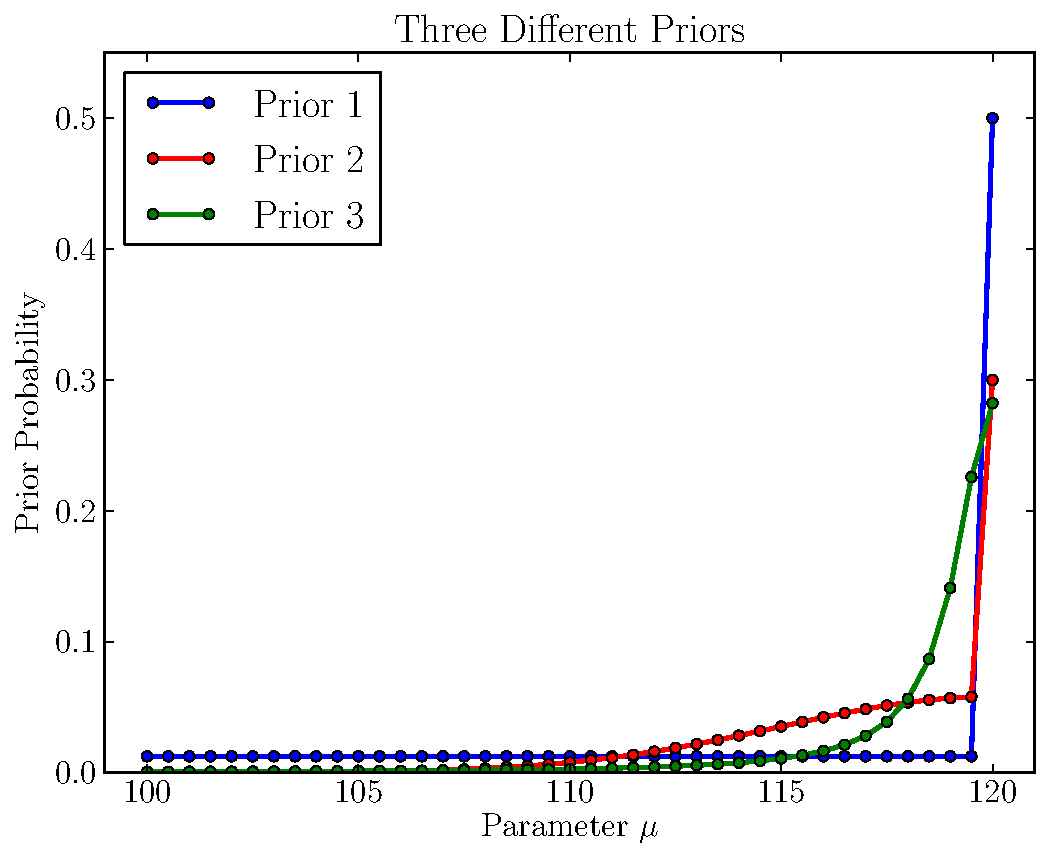
\includegraphics[scale=0.6]{Figures/testing_priors.pdf}
\caption{\it Three possible priors we could use for the blood pressure question.
All may seem ``reasonable'', and the choice can affect the results (quite
significantly in some cases). Care should be taken when choosing the prior
in hypothesis testing problems.
\label{fig:testing_priors}}
\end{center}
\end{figure}


\section{Some Terminology}
There is some alternative terminology that is widely used and is particularly
popular in Bayesian hypothesis testing (aka model selection) problems. Suppose
there were two hypotheses $H_1$ and $H_2$, and some data $x$. Now, $H_1$ and
$H_2$ might be a null and alternative hypothesis, or they might be two
particular values of the parameter, or something else. Two repetitions of Bayes' rule
for these two hypotheses are:
\begin{eqnarray}
P(H_1 | x) &=& \frac{P(H_1)p(x|H_1)}{p(x)}\\
P(H_2 | x) &=& \frac{P(H_2)p(x|H_2)}{p(x)}
\end{eqnarray}
These could also be written in words:
\begin{eqnarray}
\textnormal{posterior} &=& \frac{\textnormal{prior}\times\textnormal{likelihood}}{\textnormal{marginal likelihood}}
\end{eqnarray}

Dividing these two equations gives the {\it odds form} of Bayes' rule, which
deals with ratios of probabilities instead of probabilities themselves.
\begin{eqnarray}
\frac{P(H_1 | x)}{P(H_2|x)} &=& \frac{P(H_1)}{P(H_2)} \times
\frac{p(x|H_1)}{p(x|H_2)}\label{eq:odds_form}
\end{eqnarray}
In words, this can be written as:
\begin{eqnarray}
\textnormal{posterior odds} = \textnormal{prior odds}
\times
\textnormal{bayes factor}
\end{eqnarray}
Sometimes people talk about odds (or odds ratios, which are the same thing)
and Bayes Factors instead of about prior and
posterior probabilities. The odds tell us how plausible $H_1$ is compared to
$H_2$. For example, a posterior odds ratio of 5 means $H_1$ is 5 times as plausible
as $H_2$. Of course, odds can be greater than 1 even though probabilities
cannot be. The Bayes Factor is the ratio of the likelihoods. Results are often
quoted as Bayes Factors because that's the part of the equation where the
data is important. If you say ``The Bayes Factor for $H_1$ over $H_2$ was 10'',
then whoever you're talking to is free to apply whatever prior odds they like,
whereas if you state the posterior odds then people may wonder what your prior
odds were.

\section{Hypothesis Testing and the Marginal Likelihood}\label{sec:marginal_likelihood}
The Bayes' factor in Equation~\ref{eq:odds_form} is the ratio of likelihoods
for two hypotheses $H_1$ and $H_2$. If we wanted to calculate the Bayes Factor
for $H_0$ and $H_1$ in the blood pressure example, we could easily get the likelihood
for $H_0$ (it's right there in the Bayes' Box). But how would we get $p(x|H_1)$,
which needs to be a single number? $H_1$ is the statement $\mu = 100$ {\bf or}
$\mu = 111$ {\bf or} $\mu = 112$ and so on up to $\mu = 119$.

Imagine we had left $\mu=120$ out of our Bayes' Box and just done parameter
estimation within the context of $H_1$ (i.e. assuming, for argument's sake,
that $H_1$ is true). This would involve a {\it reduced} Bayes' Box with one
less row in it. We would end up getting some marginal likelihood
$p(x) = \sum p(\theta)p(x|\theta)$.
The key is to realise that since we are assuming $H_1$ throughout, the
marginal likelihood is really $p(x|H_1) = \sum p(\theta|H_1)p(x|\theta, H_1)$,
which is exactly the thing we need to calculate the Bayes Factor!

All of this implies
there are two mathematically equivalent ways of doing Bayesian hypothesis testing,
or model selection. One is to make a big model that includes both the null and
the alternative hypothesis. The Bayes' Box with a testing prior accomplishes this.
In most cases this is the most convenient way to do the calculations.

The other way is to do the two analyses separately. First, do parameter estimation
within the context of $H_1$. Then, do parameter estimation within the context
of $H_2$. Then, use the marginal likelihoods as if they were likelihoods, to
compare $H_1$ vs. $H_2$. This second way of calculating Bayes Factors is
most useful when the two analyses were actually done separately by different
people.

\section{Analytic Solution}
In this section we'll solve the blood pressure model selection problem
analytically. Firstly, let's write down the likelihood,
which is a product of $N$ univariate normal densities:
\begin{eqnarray}
p(\boldsymbol{x} | \mu) &=&
\prod_{i=1}^N \frac{1}{\sigma\sqrt{2\pi}}
\exp
\left[-\frac{1}{2\sigma^2}\left(x_i - \mu\right)^2\right].
\end{eqnarray}
We can rearrange this a bit, which will be useful later:
\begin{eqnarray}
p(\boldsymbol{x} | \mu) &=& \sigma^{-N}(2\pi)^{-N/2}
\exp
\left[-\frac{1}{2\sigma^2}\sum_{i=1}^N\left(x_i - \mu\right)^2\right]\\
&=& \sigma^{-N}(2\pi)^{-N/2}
\exp
\left[-\frac{1}{2\sigma^2}\left(N\bar{x^2} - 2N\mu\bar{x} + N\mu^2\right)\right]\\
&=& \sigma^{-N}(2\pi)^{-N/2}
\exp
\left[-\frac{N}{2\sigma^2}\left(\bar{x^2} + \mu^2\right) + \frac{N\mu}{\sigma^2}\bar{x}\right].\label{eq:lik_simplified}
%\sum_{i=1}^N\left(x_i^2 - 2\mu x_i + \mu^2\right)\right].
\end{eqnarray}
where $\bar{x}$ is the arithmetic mean of the data and $\bar{x^2}$ is the mean
squared value of the data. Notice that the likelihood only depends on the data
through the values of $\bar{x}$ and $\bar{x^2}$. In fact, if we're only trying
to infer $\mu$ and not $\sigma$ then the part that depends on $\bar{x^2}$
can be treated as a ``constant'', and will not affect the posterior for $\mu$.
This is why $\bar{x}$ is a sufficient statistic. If we were treating $\sigma$
as unknown as well, $\bar{x}$ and $\bar{x^2}$ would be sufficient statistics.


As we saw before, model selection problems can be solved in two different ways
(but with equivalent results). We can calculate the posterior for $\mu$ in
a way that includes both $H_0$ and $H_1$ in the calculation from the beginning
(perhaps assigning 50\% prior probability to $H_0$), or we can compute the
marginal likelihoods for $H_0$ and $H_1$ separately. In analytical calculations
the separate calculation is the most popular, so let's do it that way first.

The posterior odds ratio for $H_0$ over $H_1$ is
\begin{eqnarray}
\frac{P(H_0 | \boldsymbol{x})}{P(H_1|\boldsymbol{x})} &=& \frac{P(H_0)}{P(H_1)} \times
\frac{p(\boldsymbol{x}|H_0)}{p(\boldsymbol{x}|H_1)}\label{eq:odds_form2}.
\end{eqnarray}
If we're assigning 50\% prior probability to $H_0$ and to $H_1$, then the
prior odds ratio is $0.5 / 0.5 = 1$. Therefore we just need the two likelihoods,
$p(\boldsymbol{x} | H_0)$ and $p(\boldsymbol{x} | H_1)$. The first of these is fairly straightforward to
get, since $H_0$ implies $\mu = 120$. We just calculate the value of the
likelihood using Equation~\ref{eq:lik_simplified}, which we've already done
(it was in Table~\ref{tab:testing_prior}, albeit arbitrarily scaled). Its value
is $p(\boldsymbol{x} | H_0) = 1.638 \times 10^{-159}$.

To complete the calculation we need the value of $p(\boldsymbol{x}|H_1)$, but
this is a bit more difficult since $H_1$ doesn't correspond to a particular
value of $\mu$, but instead implies that $\mu$ is any value other than 120.
So what exactly does it mean? In the discrete situation, it's possible to
calculate $p(\boldsymbol{x}|H_1)$ by recognising that $H_1$ is equivalent to
$(\mu = 110) \textbf{ or } (\mu = 111) \textbf{ or }... (\mu = 119)$. Then
we can use the sum rule:
\begin{eqnarray}
p(\boldsymbol{x}|H_1) &=& \sum_{\mu=110}^{119} p(\mu | H_1)
p(\boldsymbol{x}|\mu, H_1).\label{eqn:discrete_evidence}
\end{eqnarray}
Since we're working analytically, we'll be replacing this marginal likelihood
with a continuous version that allows any possible $\mu$ value on the real line.
The integral for the marginal likelihood will take a form analogous to
Equation~\ref{eqn:discrete_evidence}:
\begin{eqnarray}
p(\boldsymbol{x}|H_1) &=& \int p(\mu | H_1)
p(\boldsymbol{x}|\mu, H_1) \, d\mu.\label{eqn:continuous_evidence}
\end{eqnarray}
The limits for the integration must be whatever range of $\mu$ is possible.

Recall the notion of a ``conjugate prior'' which was discussed briefly earlier
(when we used a beta prior together with a binomial sampling distribution).
This is a mathematical trick where we choose a particular kind of prior
that works together nicely with the mathematical form of the likelihood, so
that we can do our calculations and actually get an answer in closed form.
If we look at Equation~\ref{eq:lik_simplified} as a function of $\mu$, we
can see that it is an exponential of a quadratic term, which has the same
mathematical form as a gaussian.

If we make the prior for $\mu$ (given $H_1$) a normal distribution, then the
equation for the density will also be a gaussian function of $\mu$. Two
gaussian functions multiplied together become a single gaussian function, whose
integral we can do. This is the kind of thing that Bayesians used to have to
do in order to make their calculations tractable. It's okay if you wouldn't
have guessed that a normal distribution would be the conjugate prior here.

A normal prior centered at centered at $m$ with a standard deviation of $s$
has the following probability density function:
\begin{eqnarray}
p(\mu | H_1) &=& \frac{1}{s\sqrt{2\pi}}\exp
\left[-\frac{1}{2s^2}\left(\mu - m\right)^2\right]
\end{eqnarray}

Using Bayes' rule, the posterior is proportional to the prior multiplied by
the likelihood. This is all conditional on $H_1$, which we should remember
to put in the right hand side of the ``given'' sign in all of our terms:

\begin{eqnarray}
p(\mu | x, H_1) &\propto& p(\mu | H_1)p(x | \mu, H_1) \\
&\propto&
\frac{1}{s\sqrt{2\pi}}\exp
\left[-\frac{1}{2s^2}\left(\mu - m\right)^2\right]
\times
\prod_{i=1}^N \frac{1}{\sigma\sqrt{2\pi}}
\exp
\left[-\frac{1}{2\sigma^2}\left(x_i - \mu\right)^2\right]
\end{eqnarray}

